\section{Эксперименты}
В данной главе описаны эксперименты по сравнению 
производительности неспециализированного алгоритма Витерби 
против специализированного алгоритма Витерби первого и второго уровня,
а также по сравнению с реализацией из существующего решения \name{CUDAMPF} из 
подраздела~\ref{lab:CUDAMPF}.
Существующее решение \name{HMMer} из подраздела~\ref{lab:HMMer} не измерялось, так как согласно статье~\cite{cudampf} \name{CUDAMPF} превосходит \name{HMMer} более чем в 20 раз.

\subsection{Описание набора данных и оборудования}
Эксперименты выполнялись на рабочей станции с ОС Ubuntu 
20.04, четырехядерном процессоре \name{Intel Core i7-6700} с частотой 3.40 ГГц, 64 Гб оперативной памяти, видеокартой 
\name{NVI\-DIA GeForce GTX 1070} c 8 Гб памяти.

В качестве тестового набора были взяты СММ из репозитория  
проекта \name{CUDAMPF}.
Это 24 так называемых \emph{молчаливых СММ}~\cite{silentHMM}, 
размером от 100 до 2405 состояний.
Каждая из этих молчаливых СММ описывает вероятностный фильтр \name{MSV}, то есть СММ, специфичную для бионформатики.
Эти СММ отличаются от СММ, описанных в разделе~\ref{lab:HMM} 
тем, что состояния могут не создавать наблюдения.
Из-за этого отличия алгоритм Витерби из 
раздела~\ref{lab:Viterbi} не будет работать корректно.
Реализация алгоритма Витерби в \name{CUDAMPF} адаптирована для работы с \name{MSV}.
Данные молчаливые СММ из репозитория \name{CUDAMPF} можно использовать 
для моделирования вычислительной нагрузки.
Чтобы ранее описанные варианты алгоритма Витерби могли 
работать с данными из молчаливой СММ, был разработан 
конвертер, который по молчаливой СММ создает СММ с теми же 
состояниями и, по возможности, сохраняет переходы между ними, 
либо добавляет новые переходы, если состояние не создавало 
наблюдений.
Количество возможных наблюдений, т.е. $K$, равно 20.
На рисунке~\ref{HMM_mean} приведена график зависимости количества СММ, используемых в базе данных \name{PFAM} версии 34.0, от количества состояний в этих моделях.
\begin{figure}[h!]
  \centering
  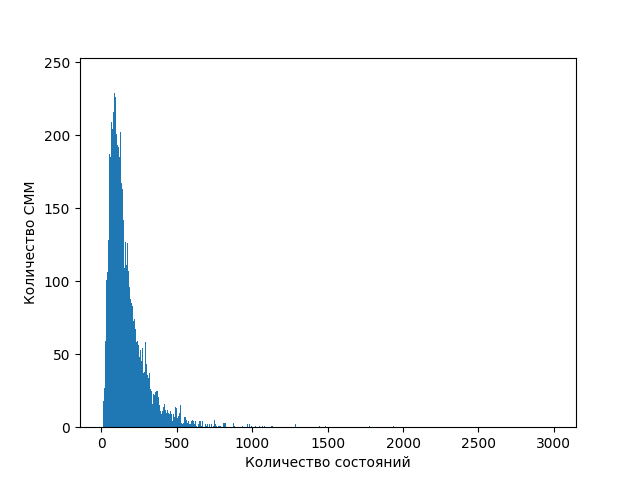
\includegraphics[width=\columnwidth]{mean_HMM.png}
  \caption{Распределение количества СММ от количества состояний}
  \label{HMM_mean}
\end{figure}

Были подготовлены следующие наборы последовательностей наблюдений:
\begin{itemize}
	\item 3 последовательности по 3500 наблюдений;
	\item 3 последовательности по 7000 наблюдений;
	\item 16 последовательностей размером от 38 до 7096;
	\item 50 последовательностей по 3500 наблюдений.
\end{itemize}
Первый, второй и четвертый наборы были искусственно сгенерированы, в то время 
как третий был взят из БД \name{PFAM} и 
приведен к формату \emph{ess}, который описан в 
разделе~\ref{lab:formats}.


\subsection{Анализ результатов}
Для получения времени выполнения каждая реализация алгоритма 
Витерби запускалась 10 раз, и из этих результатов бралась 
медиана.
Измерялось время обработки всего набора последовательностей при зафиксированной СММ конкретной реализацией.
Если реализация специализированная, то также измерялось время, необходимое на выполнение специализации.

Для реализации с использованием \name{SuiteSparse:GraphBLAS} были получены следующие результаты, представленные на рисунках~\ref{3500_SS},~\ref{7000_SS},~\ref{RW_SS},
~\ref{50_SS} и~\ref{Spec_time_SS}.
Использовались специализированные версии первого и второго уровня, для специализированной версии третьего уровня не хватило оперативной памяти.
Специализация второго уровня сильно медленнее других реализаций, поэтому она не отображена на рисунках.
В таблице~\ref{runtime} указано общее время обработки с учётом затрат на специализацию.

%\begin{tabular}{c|c|c|c|c}%
%    \bfseries Состояний & \bfseries CUDAMPF & \bfseries неспец. & \bfseries Ур.1 & \bfseries Ур.2
%    \csvreader[head to column names]{3_3500.csv}{}% use head of csv as column names
%    {\\\hline\States & \CUDAMPF & \GraphBLAS & \csvcolvi & \csvcolviii}% specify your coloumns here
%\end{tabular}

\begin{figure}[!h]
\centering
	\begin{tikzpicture}
	\begin{axis}[
     	  title={},
          axis x line=bottom,
          axis y line=left,
          xlabel={Кол-во состояний в СММ},
          ylabel={Время, мс},
          legend pos=outer north east]
		\addplot table [x=States, y=CUDAMPF, col sep=comma] {3_3500.csv};
		\addplot table [x=States, y=GraphBLAS, col sep=comma] {3_3500.csv};
		\addplot table [x=States, y=GraphBLAS_spec_1, col sep=comma] {3_3500.csv};
%		\addplot table [x=States, y=GraphBLAS_spec_2, col sep=comma] {3_3500.csv};
       	\legend{CUDAMPF, неспец., ур. 1 спец., ур. 2 спец.}
	\end{axis}
    \end{tikzpicture}
    \caption{GraphBLAS, 3 x 3500 наблюдений, меньше --- лучше}
\label{3500_SS}
\end{figure}

\begin{figure}[h!]
\centering
	\begin{tikzpicture}
	\begin{axis}[
	      title={},
          axis x line=bottom,
          axis y line=left,
          xlabel={Кол-во состояний в СММ},
          ylabel={Время, мс},
          legend pos=outer north east]
        \addplot table [x=States, y=CUDAMPF, col sep=comma] {3_7000.csv};
		\addplot table [x=States, y=GraphBLAS, col sep=comma] {3_7000.csv};
		\addplot table [x=States, y=GraphBLAS_spec_1, col sep=comma] {3_7000.csv};
       	\legend{CUDAMPF, неспец., ур. 1 спец.}
	\end{axis}
    \end{tikzpicture}
    \caption{GraphBLAS, 3 х 7000 наблюдений, меньше --- лучше}
\label{7000_SS}
\end{figure}

\begin{figure}[h!]
\centering
	\begin{tikzpicture}
	\begin{axis}[
	      title={},
          axis x line=bottom,
          axis y line=left,
          xlabel={Кол-во состояний в СММ},
          ylabel={Время, мс},
          legend pos=outer north east]
        \addplot table [x=States, y=CUDAMPF, col sep=comma] {covid-19.csv};
		\addplot table [x=States, y=GraphBLAS, col sep=comma] {covid-19.csv};
		\addplot table [x=States, y=GraphBLAS_spec_1, col sep=comma] {covid-19.csv};
       	\legend{CUDAMPF, неспец., ур. 1 спец.}
	\end{axis}
    \end{tikzpicture}
    \caption{GraphBLAS, набор данных из БД \name{PFAM}, меньше --- лучше}
\label{RW_SS}    
\end{figure}

\begin{figure}[h!]
\centering
	\begin{tikzpicture}
	\begin{axis}[
	      title={},
          axis x line=bottom,
          axis y line=left,
          xlabel={Кол-во состояний в СММ},
          ylabel={Время, мс},
          legend pos=outer north east]
        \addplot table [x=States, y=CUDAMPF, col sep=comma] {50_3500.csv};
		\addplot table [x=States, y=GraphBLAS, col sep=comma] {50_3500.csv};
		\addplot table [x=States, y=GraphBLAS_spec_1, col sep=comma] {50_3500.csv};
       	\legend{CUDAMPF, неспец., ур. 1 спец.}
	\end{axis}
    \end{tikzpicture}
    \caption{GraphBLAS, 50 х 3500 наблюдений, меньше --- лучше}
\label{50_SS}
\end{figure}

\begin{figure}[h!]
\centering
	\begin{tikzpicture}
	\begin{axis}[
	      title={},
          axis x line=bottom,
          axis y line=left,
          xlabel={Кол-во состояний в СММ},
          ylabel={Время, мс},
          legend pos=outer north east]
		\addplot table [x=States, y=GraphBLAS_spec_1_prep, col sep=comma] {50_3500.csv};
		\addplot table [x=States, y=GraphBLAS_spec_2_prep, col sep=comma] {50_3500.csv};
       	\legend{ур. 1 спец., ур. 2 спец.}
	\end{axis}
    \end{tikzpicture}
    \caption{GraphBLAS, время на специализацию, меньше --- лучше}
\label{Spec_time_SS}
\end{figure}

\begin{table}[h!]
  \centering
  \begin{tabular}{||c c c c c||} 
    \hline
    & CUDAMPF & неспец. & Ур. 1 & Ур. 2 \\ [0.5ex] 
    \hline\hline
    3 x 3500 & 4854 & 10765 & 8062 & 215329 \\ 
    \hline
    3 x 7000 & 9209 & 21062 & 16152 & 387464 \\
    \hline
    Набор из \name{PFAM} & 8796 & 15864 & 12036 & 298269 \\
    \hline
    50 x 3500 & 103036 & 176263 & 134259 & 2921104 \\
    \hline
  \end{tabular}
  \caption{GraphBLAS, общее время обработки с учетом затрат времени на специализацию, мс}
  \label{runtime}
\end{table}

Как можно видеть из графиков и таблицы, специализированная версия первого уровня превосходит неспециализированную.
Стоит отметить, что специализация первого уровня хуже \name{CUDAMPF} примерно в 1,5-2 раза.

При измерении специализированных реализаций с использованием библиотеки \name{CUSP} были получены следующие результаты, которые представлены на рисунках~\ref{3500_CUSP},~\ref{7000_CUSP},~\ref{RW_CUSP},~\ref{50_CUSP} и~\ref{Spec_time_CUSP}, а также в таблице~\ref{runtime_CUSP}.
Здесь использовалась специализация только первого уровня, так как на видеокарте не хватило памяти для специализации второго и далее уровней.
\begin{figure}[h!]
\centering
	\begin{tikzpicture}
	\begin{axis}[
	      title={},
          axis x line=bottom,
          axis y line=left,
          xlabel={Кол-во состояний в СММ},
          ylabel={Время, мс},
          legend pos=outer north east]
        \addplot table [x=States, y=CUDAMPF, col sep=comma] {3_3500.csv};
		\addplot table [x=States, y=CUSP, col sep=comma] {3_3500.csv};
		\addplot table [x=States, y=CUSP_spec_1, col sep=comma] {3_3500.csv};
       	\legend{CUDAMPF, неспец., ур. 1 спец.}
	\end{axis}

    \end{tikzpicture}
    \caption{CUSP, 3 x 3500 наблюдений, меньше --- лучше}
\label{3500_CUSP}
\end{figure}

\begin{figure}[h!]
\centering
	\begin{tikzpicture}
	\begin{axis}[
	      title={},
          axis x line=bottom,
          axis y line=left,
          xlabel={Кол-во состояний в СММ},
          ylabel={Время, мс},
          legend pos=outer north east]
        \addplot table [x=States, y=CUDAMPF, col sep=comma] {3_7000.csv};
		\addplot table [x=States, y=CUSP, col sep=comma] {3_7000.csv};
		\addplot table [x=States, y=CUSP_spec_1, col sep=comma] {3_7000.csv};
       	\legend{CUDAMPF, неспец., ур. 1 спец.}
	\end{axis}

    \end{tikzpicture}
    \caption{CUSP, 3 х 7000 наблюдений, меньше --- лучше}
\label{7000_CUSP}
\end{figure}

\begin{figure}[h!]
\centering
	\begin{tikzpicture}
	\begin{axis}[
	      title={},
          axis x line=bottom,
          axis y line=left,
          xlabel={Кол-во состояний в СММ},
          ylabel={Время, мс},
          legend pos=outer north east]
        \addplot table [x=States, y=CUDAMPF, col sep=comma] {covid-19.csv};
		\addplot table [x=States, y=CUSP, col sep=comma] {covid-19.csv};
		\addplot table [x=States, y=CUSP_spec_1, col sep=comma] {covid-19.csv};
       	\legend{CUDAMPF, неспец., ур. 1 спец.}
	\end{axis}

    \end{tikzpicture}
    \caption{CUSP, набор данных из БД \name{PFAM}, меньше --- лучше}
\label{RW_CUSP}    
\end{figure}

\begin{figure}[h!]
\centering
	\begin{tikzpicture}
	\begin{axis}[
	      title={},
          axis x line=bottom,
          axis y line=left,
          xlabel={Кол-во состояний в СММ},
          ylabel={Время, мс},
          legend pos=outer north east]
        \addplot table [x=States, y=CUDAMPF, col sep=comma] {50_3500.csv};
		\addplot table [x=States, y=CUSP, col sep=comma] {50_3500.csv};
		\addplot table [x=States, y=CUSP_spec_1, col sep=comma] {50_3500.csv};
       	\legend{CUDAMPF, неспец., ур. 1 спец.}
	\end{axis}
    \end{tikzpicture}
    \caption{CUSP, 50 x 3500 наблюдений, меньше --- лучше}
\label{50_CUSP}
\end{figure}

\begin{figure}[h!]
\centering
	\begin{tikzpicture}
	\begin{axis}[
	      title={},
          axis x line=bottom,
          axis y line=left,
          xlabel={Кол-во состояний в СММ},
          ylabel={Время, мс},
          legend pos=outer north east]
		\addplot table [x=States, y=CUSP_spec_1_prep, col sep=comma] {50_3500.csv};
       	\legend{ур. 1 спец.}
	\end{axis}
    \end{tikzpicture}
    \caption{CUSP, время на специализацию, меньше --- лучше}
\label{Spec_time_CUSP}
\end{figure}


\begin{table}[h!]
  \centering
  \begin{tabular}{||c c c c||} 
    \hline
    & CUDAMPF & неспец. & Ур. 1 \\ [0.5ex] 
    \hline\hline
    3 x 3500 & 4854 & 358002 & 201089 \\ 
    \hline
    3 x 7000 & 9209 & 713968 & 400829 \\
    \hline
    Набор из \name{PFAM} & 8796 & 535354 & 301435 \\
    \hline
    50 x 3500 & 103036 & 5983963 & 3339231 \\
    \hline
  \end{tabular}
  \caption{CUSP, общее время обработки с учетом затрат времени на специализацию, мс}
  \label{runtime_CUSP}
\end{table}

Исходя из полученных результатов, можно сделать вывод, что, 
как и в случае с реализациями с использованием 
\name{GraphBLAS}, при специализации первого уровня
снижается время обработки последовательностей.
В конкретном случае, реализации оказались не такими 
производительными по сравнению с \name{CUDAMPF} и 
\name{GraphBLAS}.
Причиной этого являются особенности реализации библиотеки 
\name{CUSP}.
\achtung{Нормально попрофилировать}

Анализируя данные экспериментов, стоит отметить, что 
специализированный алгоритм Витерби первого уровня производительнее, 
чем неспециализированная версия, то есть специализация дает прирост 
по скорости обработке последовательностей наблюдений за счет 
уменьшения количества матричных операций.
При повышении уровня специализации на второй наблюдается 
ухудшение производительности.
\achtung{Указать на то, что лучше в плане инженерии.}

\newpage